% 第 8 周交付物：最终项目报告（中文版） —— 编译方式：XeLaTeX
\documentclass[11pt]{ctexart}
\usepackage[a4paper, margin=2.4cm]{geometry}
\usepackage{amsmath, amssymb}
\usepackage{booktabs}
\usepackage{graphicx}
\usepackage[hidelinks]{hyperref}
\usepackage{enumitem}
\setlist{nosep}
\usepackage{parskip}
\usepackage{float}

\title{\textbf{Advanced Chooser Option Pricing Model\\ with Real-World Data \& Machine Learning}\\
\Large 最终项目报告}
\author{佟铸城（Zhucheng Tong）}
\date{2026 年 9 月 \quad（项目周期：2026-07 至 2026-09，第 1--8 周）}

\begin{document}
\maketitle

\begin{abstract}
本项目围绕 JPM 标的的 simple chooser option 构建了一套数据驱动的定价体系：复现并三角验证了 Rubinstein（1991）闭式解与蒙特卡洛定价，在 1310 个交易日的真实数据上以“事后真值”口径量化了 BSM 常数波动率假设的代价（最优回望校准的相对误差约 35\%），继而在严格的样本外协议（净化时序切分、walk-forward 重训、测试集单次开封）下检验了两条机器学习增强路线。核心结论：（1）失效模式随波动率估计器记忆长度分化，无单一回望窗口全状态占优；（2）在仅含约一个半波动率状态周期的训练数据上，ML 修正无法稳健标定，所有配置在测试集上不敌 EWMA 锚定基线——该负结果经六项审计确认为科学结论而非实现缺陷；（3）正确的融合形态是“随机过程出框架、机器学习学残差”的 1+1 结构而非二选一。最终交付物为一个 Streamlit 双定价工具：主定价采用全程最稳健的 EWMA 锚定 BSM，ML 修正价附样本外警示作参考。
\end{abstract}

{\small\setlength{\parskip}{0pt}\tableofcontents}
\newpage

\section{项目概述}
Chooser option 赋予持有人在选择日 $t_1$ 决定期权为欧式 call 或 put 的权利（共同行权价 $K$、到期日 $T_2$），适用于方向不明但预期大波动的场景（财报、FOMC 等）。项目目标：（1）复现参考论文（Huang, Wang \& Wan, 2021）的 BSM 定价并以真实数据验证；（2）多维数据采集与特征工程；（3）机器学习优化波动率预测与定价；（4）量化 ML 与传统 BSM 的对比；（5）交付可部署定价工具。八周执行路线：数据管道（W1--2）$\to$ 复现与基线（W3--4）$\to$ ML 两路线（W5--6）$\to$ 工具与交付（W7--8）。

\section{数据体系（第 1--2 周）}
\textbf{来源}：Yahoo Finance（JPM 日线含股息、\^{}GSPC、\^{}VIX、国债收益率指数，主源）、FRED（DGS3MO/DGS1/DGS10/FEDFUNDS/T10Y2Y）、Alpha Vantage（备用/实时）；窗口 2018--2024 日频，经导师确认以 VIX 派生特征替代新闻情绪数据、以蒙特卡洛替代 CME 成交价。\textbf{清洗}：NYSE 交易日历对齐、按缺失机制区分的填充（利率时间插值、政策利率阶梯填充）、IQR 离群值\textbf{标记但保留}（全部对应真实市场事件，审计留档）。\textbf{特征}：18 个，分收益/波动率、股息、利率、市场背景、情绪（VIX 派生，0--1 情绪分 = 滚动 252 日分位；双重角色控制：原始水平=波动率、标准化变换=情绪）五族。\textbf{自动化}：GitHub Actions 每周五收盘后自动采集$\to$预处理$\to$提交，研究窗口与数据新鲜度经环境变量解耦。

\section{Chooser 定价理论与复现（第 3 周）}
利用 put--call parity，simple chooser 在 $t_1$ 的价值 $\max(C,P)$ 可分解为静态组合：一份 $(K,T_2)$ call 加 $e^{-q\tau}$ 份 $(Ke^{-(r-q)\tau},t_1)$ put（$\tau=T_2-t_1$），故 BSM 下存在闭式解。以论文 Table 2 参数（$S_0=156.7$，$K=150$，$r=0.15\%$，$\sigma=28.2\%$，$q=2.33\%$，$t_1=0.5$，$T_2=1$）复现：

\begin{center}
\small
\begin{tabular}{lr}
\toprule
闭式解（两种独立实现，差异 $7\times10^{-15}$） & \textbf{\$29.1299} \\
蒙特卡洛（条件 MC，100 万路径） & \$29.1426 $\pm$ 0.0165 \\
vanilla call / put / straddle & \$18.69 / \$15.37 / \$34.06 \\
\bottomrule
\end{tabular}
\end{center}

正确性由三角测量确立：双解析实现互查、双 MC 估计量（$1/\sqrt{n}$ 收敛）、无套利排序 $\max(C,P)<\text{chooser}<\text{straddle}$。条件 MC（选择日价值解析化）使标准误降至终值模拟的 54\%。论文的四条敏感性方向全部复现；两项超出论文的增量：（a）$t_1$ 敏感性（论文自认未竟）——价值从 $\max(C,P)$ 单调过渡到 straddle；（b）论文 moneyness 选择规则（理性临界点应为 $S^*=Ke^{(q-r)\tau}$ 而非 $K$）的代价量化：2021 年零利率下仅 6bp、$r=10\%$ 时放大至 60bp，真实日期复检 14.4bp $\to$ 32.2bp——近似是否无害是状态依赖的命题。

\begin{figure}[H]
\centering
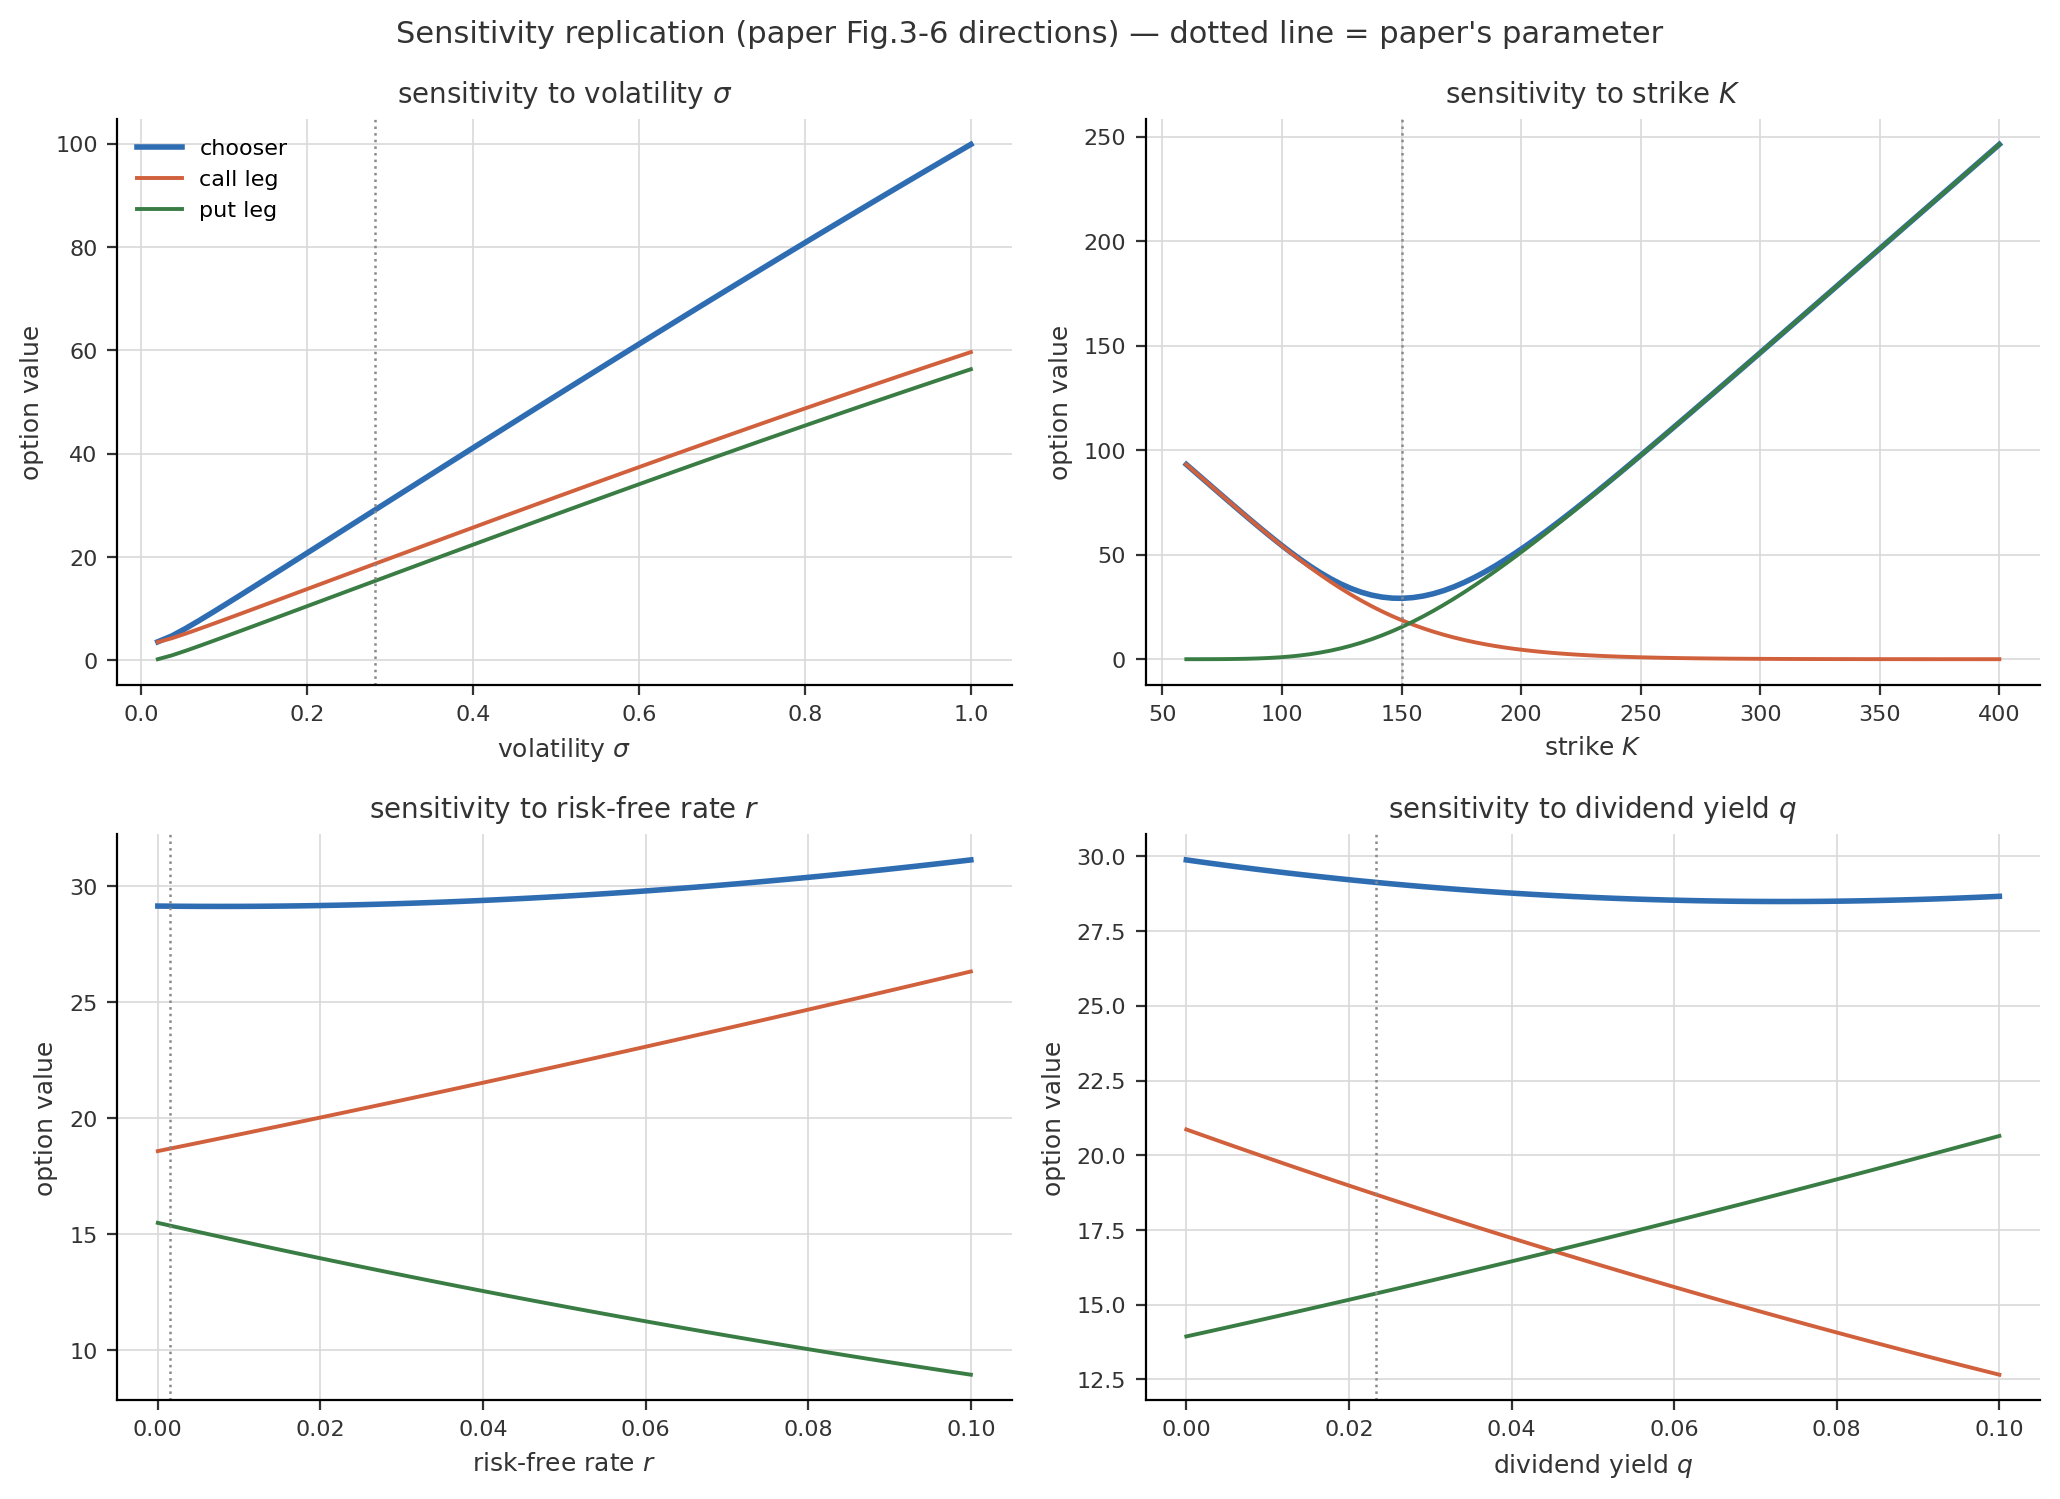
\includegraphics[width=0.9\textwidth]{../week3/figures/sensitivity_panels.png}
\caption{敏感性复现（$\sigma$/$K$/$r$/$q$；虚线为论文参数点）：方向与论文 Fig.3--6 一致，chooser 对 $K$ 呈 U 形}
\end{figure}

\begin{figure}[H]
\centering
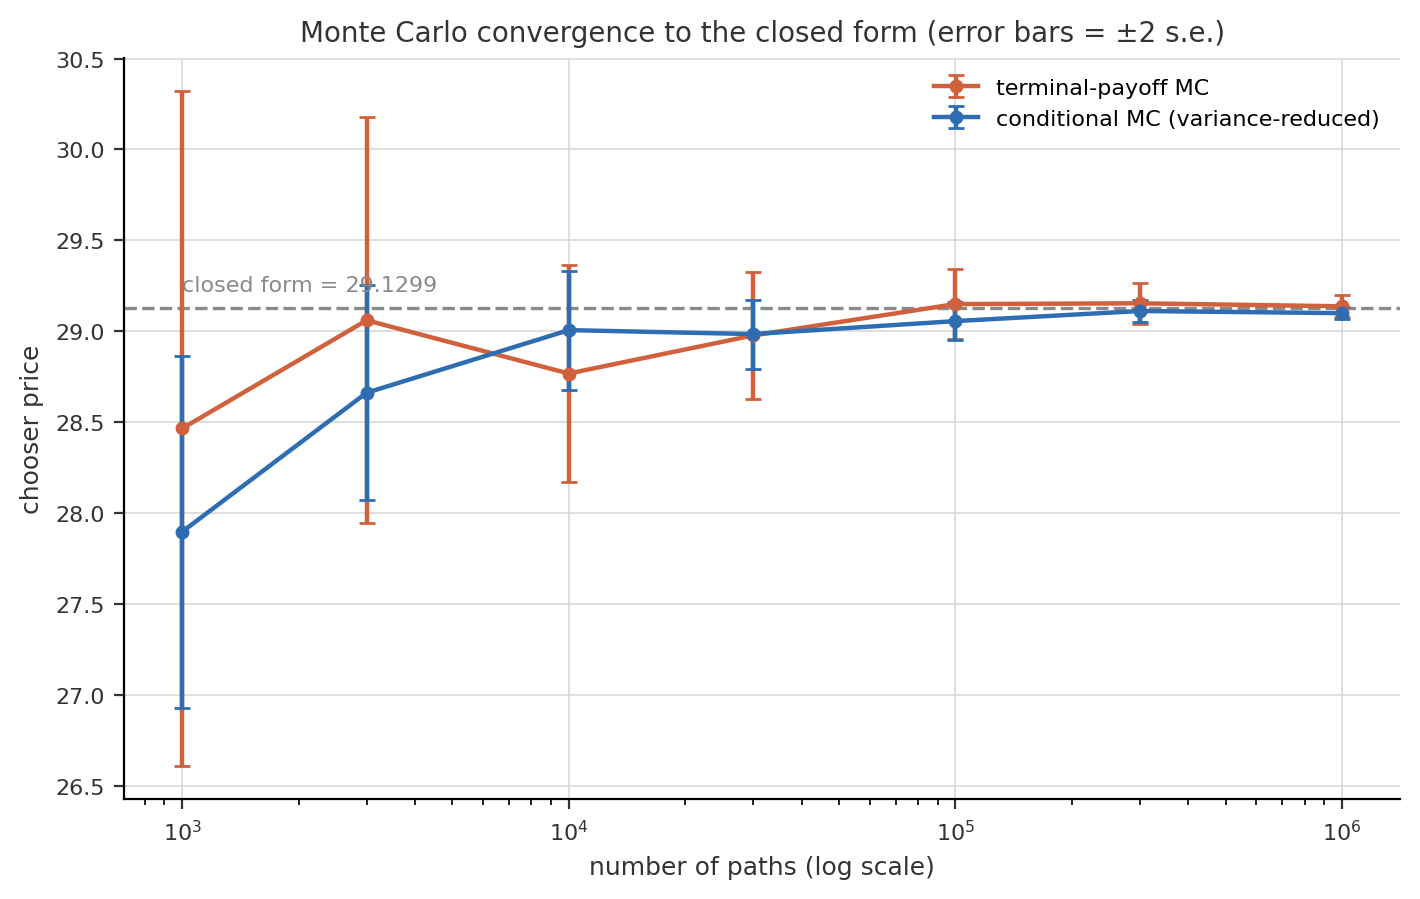
\includegraphics[width=0.58\textwidth]{../week3/figures/convergence.png}
\caption{MC 收敛性：条件 MC 与终值模拟均以 $1/\sqrt{n}$ 收敛于闭式解}
\end{figure}

\section{基线评估：常数波动率假设的代价（第 4 周）}
评估设计采用\textbf{事后真值（oracle）}口径：逐日发行 ATM 1 年期 chooser，回望校准价（$\sigma$ 取各回望估计器）与“用存续期内实际实现波动率”的 oracle 价对比——误差唯一地归因于常数波动率假设。样本 1310 个交易日（2019-10 至 2024-12）。

\begin{center}
\small
\begin{tabular}{lrrrrr}
\toprule
\textbf{$\sigma$ 估计器} & \textbf{MAE(\$)} & \textbf{相对 MAE} & \textbf{平静期} & \textbf{恐慌期} & \textbf{综合分} \\
\midrule
21 日已实现 & 9.80 & 36.1\% & 9.31 & 11.38 & 1.067 \\
63 日已实现 & 9.76 & 37.4\% & 9.47 & 10.70 & 0.994 \\
252 日已实现 & 10.37 & 41.7\% & \textbf{10.94} & 8.55 & 0.982 \\
EWMA($\lambda$=0.94) & \textbf{9.44} & \textbf{35.3\%} & 9.01 & 10.83 & 1.000（参照）\\
\bottomrule
\end{tabular}
\end{center}

关键发现：（1）最优回望校准的代价仍达价格的 \textbf{35\%}；（2）\textbf{失效模式随记忆长度分化}——快估计器（21日/EWMA）在恐慌期追高失效，252 日慢估计器在危机后的平静期拖尾失效（2021 年：\$10.34 vs 21 日的 \$6.13），无单一窗口全状态占优；（3）所有回望基线对 oracle 价格的 $R^2$ 为负（约 $-1.1$），解释力不如常数均值——常数波动率失效的最尖锐表述；（4） 2019 年尾段误差（\$31.8）源于标签窗口内的 COVID 崩盘，为任何回望方法（含 ML）设定了不可约的期望上限。
\begin{figure}[H]
\centering
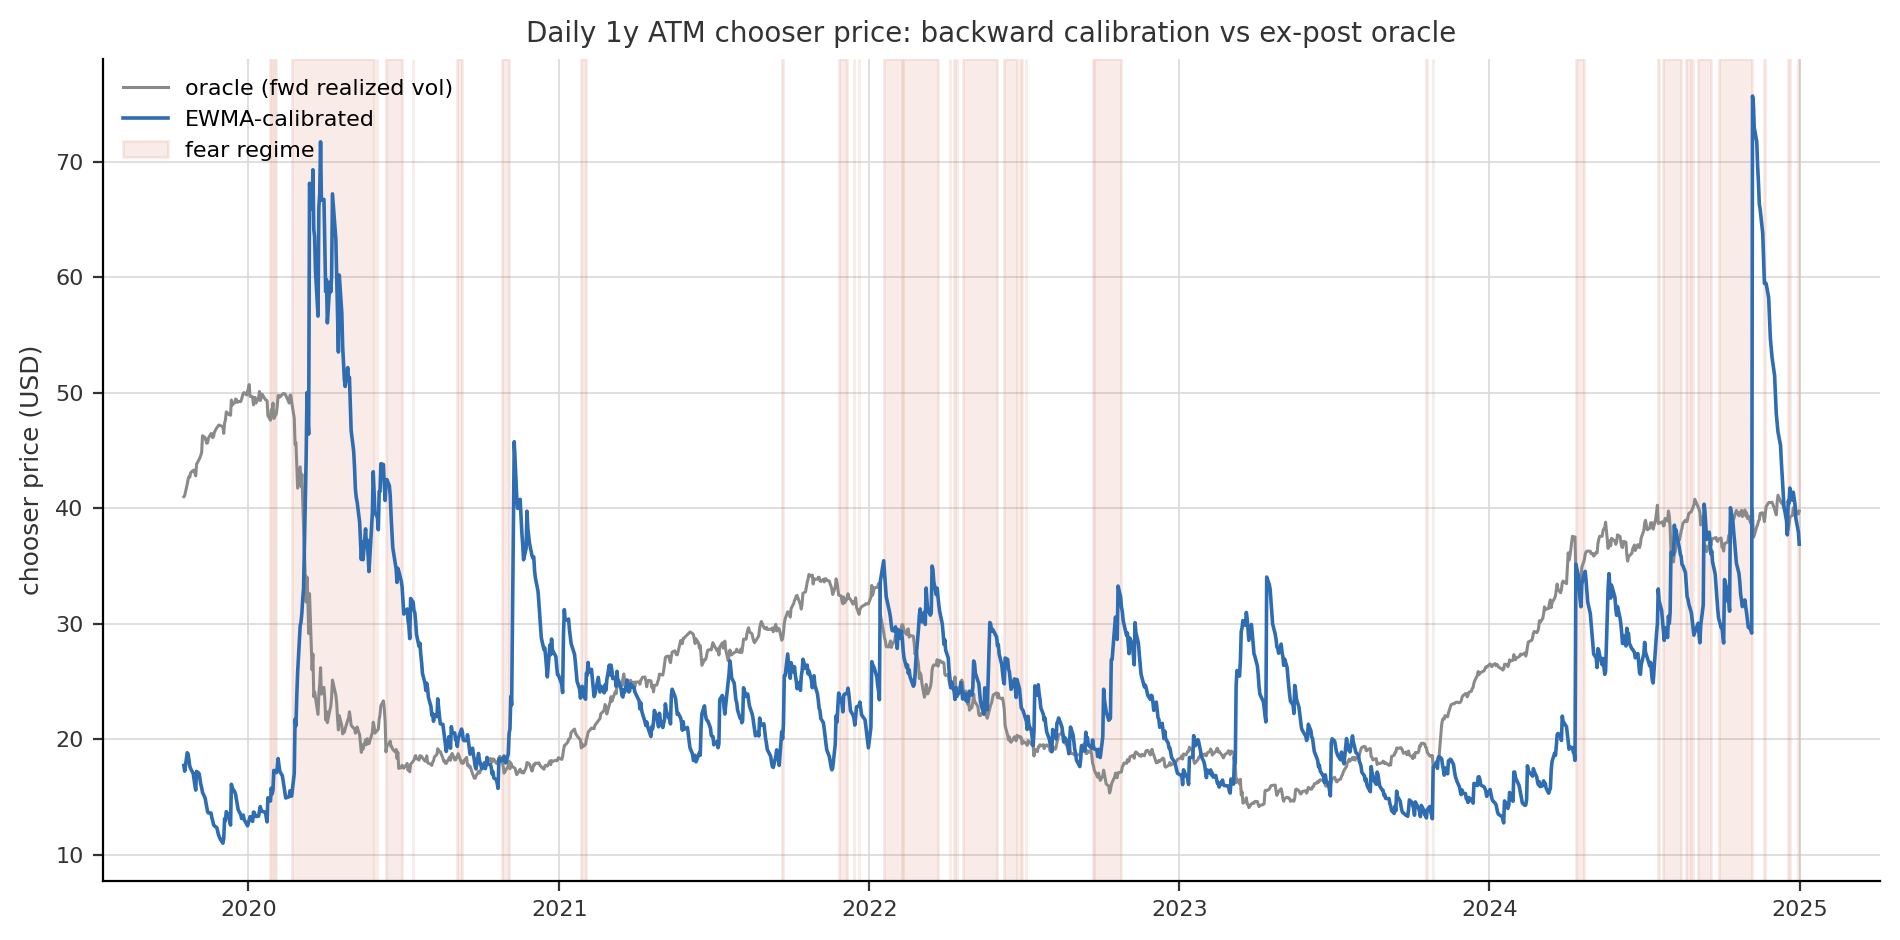
\includegraphics[width=0.94\textwidth]{../week4/figures/rolling_price.png}
\caption{逐日定价：EWMA 回望校准（蓝） vs 事后真值（灰），阴影为恐慌状态——2020 年初灰线先行抬升而蓝线浑然不觉，即 BSM 危机前低估、危机后高估}
\end{figure}

\begin{figure}[H]
\centering
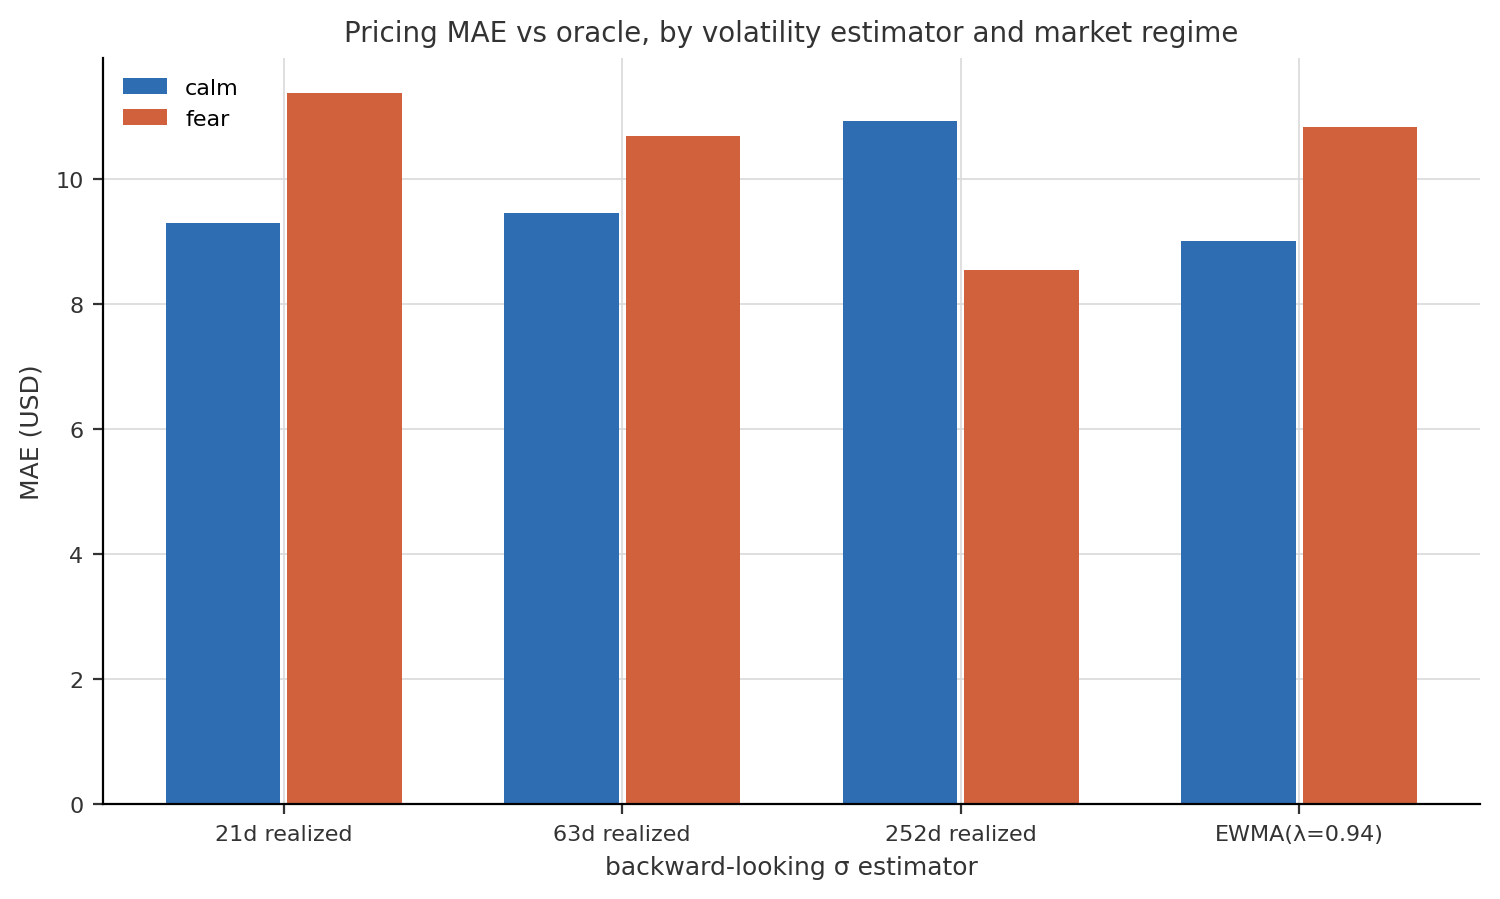
\includegraphics[width=0.6\textwidth]{../week4/figures/mae_by_regime.png}
\caption{分状态 MAE：快估计器恐慌期更差、252 日估计器平静期更差}
\end{figure}

\subsection{评估指标体系（应导师要求扩展，全项目同一把尺）}
\begin{center}
\small
\begin{tabular}{llp{6.6cm}r}
\toprule
\textbf{指标族} & \textbf{指标} & \textbf{衡量什么} & \textbf{权重} \\
\midrule
平均精度 & MAE / RMSE / MedAE & 常规误差；中位数对极端日不敏感 & 0.35 \\
尾部/稳健 & P95AE / 分状态最差 MAE & 最差 5\% 交易日；不许牺牲某一状态换平均 & 0.30 \\
方向偏差 & $|$Bias$|$ & 系统性高估/低估，对报价比对称噪声更危险 & 0.10 \\
解释力 & $1-R^2$ & 相对“永远猜均值”的改进 & 0.10 \\
可用率 & $1-$Hit10 & 相对误差 $<10\%$ 的天数占比 & 0.15 \\
\bottomrule
\end{tabular}
\end{center}
综合分 $=\sum_i w_i\,\mathrm{metric}_i(m)/\mathrm{metric}_i(\text{EWMA})$，参照模型恒为 1、$<1$ 即胜基线；比值化使新增模型无需重新归一，并附等权/精度导向/稳健导向三种替代权重的排名敏感性检验。

\section{机器学习增强：设计、协议与结果（第 5--6 周）}

\subsection{防泄漏协议}
70/15/15 时序切分 + \textbf{净化}（训练尾部删 252 行，标签前视窗不越界）+ 测试集（2024-03 至 2024-12）\textbf{单次开封}（全部选择只用验证集，审计断言保证选择日志零测试信息）+ walk-forward 季度重训（逐块净化与 scaler 重拟合）。

\subsection{设计演进：从水平目标到锚定目标}
直接预测波动率水平的七个初版模型（Ridge/RF/GBDT/LSTM $\times$ 两路线）在验证集\textbf{全军覆没}（综合分 2.0--3.7，统一正偏差 $+14$ 至 $+26$ 美元）：COVID 主导的训练窗遇上低波动验证窗，树模型无法输出低于训练所见的值。修正为\textbf{锚定目标} $y=\ln(\sigma_{oracle}/\sigma_{EWMA})$（输出 0 恒等还原基线，审计断言逐日验证）后，锚定 Ridge 在验证集综合分 0.567、首个全面击败基线——锚定与第 3 周条件 MC 同源：\textbf{把已知结构从任务中剥离，学习只留给残差}。

\begin{figure}[!htb]
\centering
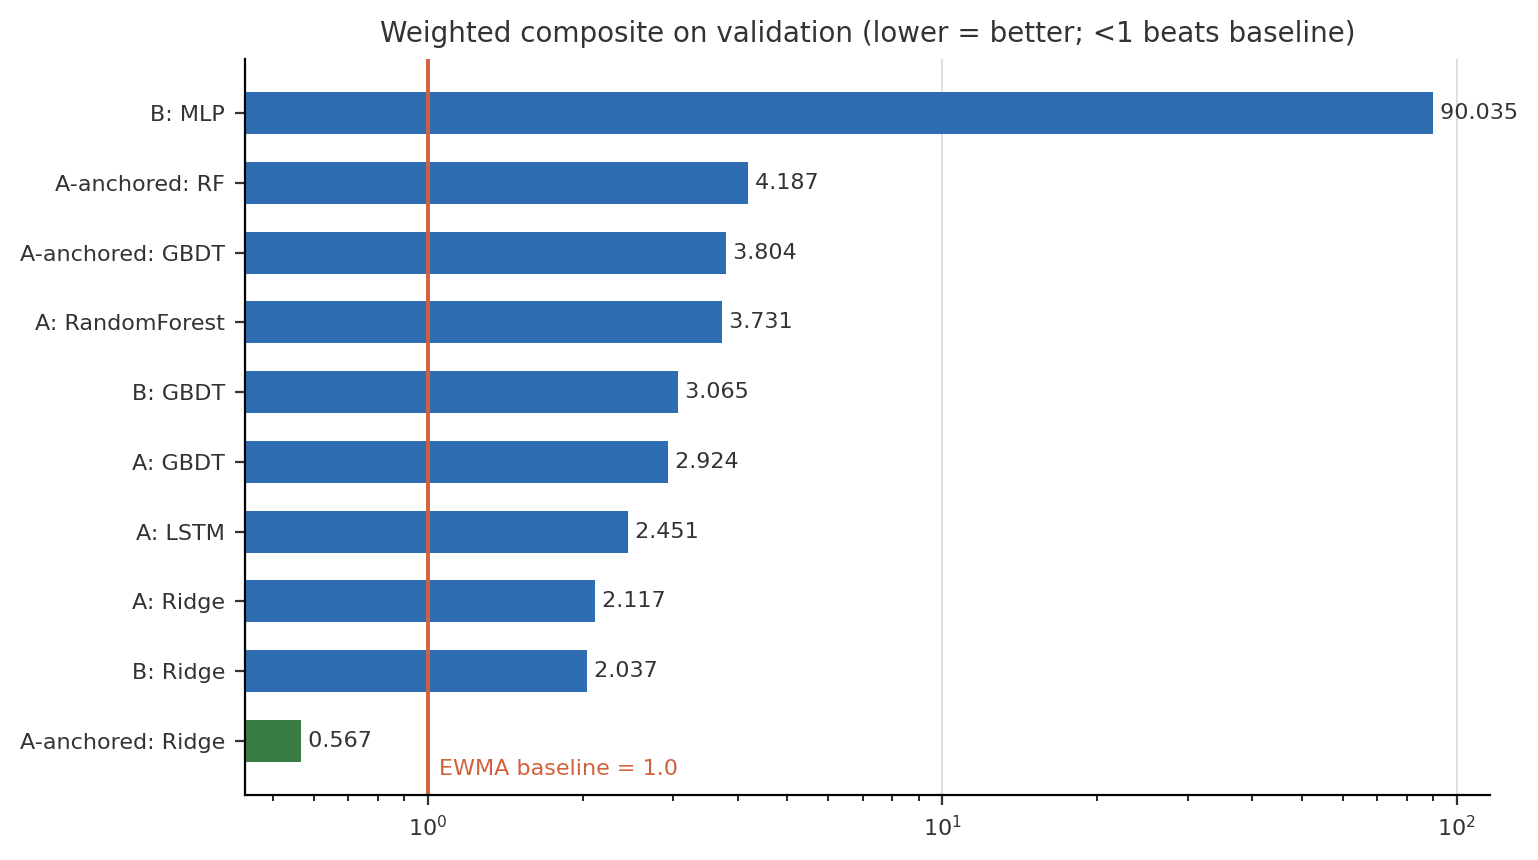
\includegraphics[width=0.72\textwidth]{../week5/figures/val_composite.png}
\caption{第 5 周验证集综合分（对数轴）：锚定 Ridge（绿，0.567）为唯一 $<1$ 者；直接预测水平的模型全部大幅劣于基线}
\end{figure}

\subsection{调参（仅用验证集）}
\begin{center}
\small
\begin{tabular}{llr}
\toprule
\textbf{模型} & \textbf{选中超参数} & \textbf{验证 MAE(\$)} \\
\midrule
A: Ridge / B: Ridge & $\alpha=10$ / $\alpha=10$ & 10.77 / 11.09 \\
A: RandomForest & max\_depth=4 & 20.35 \\
A: GBDT / B: GBDT & lr=0.03，200 轮 / lr=0.05，300 轮 & 24.17 / 23.33 \\
A: LSTM（固定配置） & hidden 32 & \textbf{2.82} \\
B: MLP（鲁棒化） & （64,32），输入裁剪 & 12.12 \\
\bottomrule
\end{tabular}
\end{center}

\subsection{最终样本外结果：一个如实报告的负结果}
经调参与 walk-forward 后在测试集单次评估：

\begin{center}
\small
\begin{tabular}{lrrrr}
\toprule
& \textbf{MAE(\$)} & \textbf{Bias} & \textbf{Hit10} & \textbf{综合分} \\
\midrule
\textbf{EWMA 基线} & \textbf{8.51} & $-3.4$ & \textbf{26.8\%} & \textbf{1.000} \\
最优 ML（鲁棒 MLP） & 14.75 & $+14.3$ & 13.6\% & 2.020 \\
验证集冠军（LSTM，val MAE 2.82） & 17.07 & $+16.6$ & 13.6\% & 2.492 \\
其余五个配置 & 20.5--22.0 & $+20$ 上下 & $\leq10.6\%$ & 2.56--2.83 \\
\bottomrule
\end{tabular}
\end{center}

\textbf{没有任何 ML 配置在测试集上击败 EWMA 基线}（四种权重方案下均然）。归因三条：（1）锚定比率目标具强低频状态自相关，训练数据仅含约一个半状态轮换，模型学到的是“上一个状态”；（2）测试期全部标签窗口覆盖 2025-04 崩盘（不可预见，EWMA 胜在不试图预测）；（3）事后诊断（如实标注、未用于选择）表明第 5 周验证集胜利部分源于训练分布与验证需求的巧合——\textbf{单一验证窗的胜利不构成部署证据}。验证集冠军 LSTM 的测试劣化（2.82 $\to$ 17.07）是教科书式验证集过拟合实例。SHAP 显示模型学到干净的均值回复逻辑（方向正确），失败在幅度不可标定——瓶颈是数据中可辨认的状态样本数，而非算法。该负结果与“单纯时序暴力拟合不如定价模型推导精确”的判断一致，并直接决定了工具的定价策略。

\begin{figure}[H]
\centering
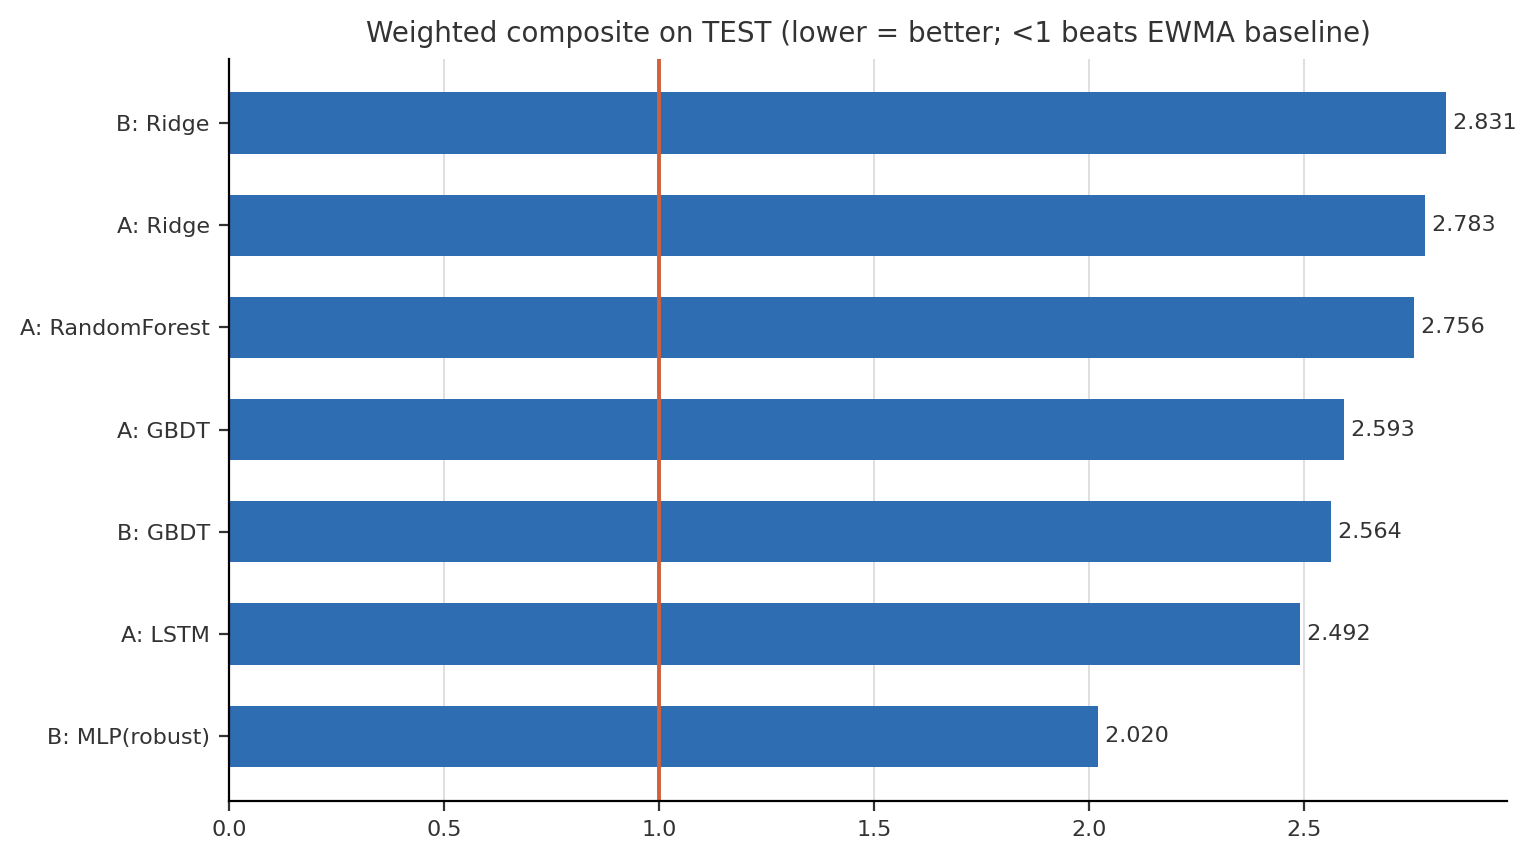
\includegraphics[width=0.7\textwidth]{../week6/figures/test_composite.png}
\caption{测试集综合分：全部 ML $>1$，EWMA 基线四种权重方案下均胜出}
\end{figure}

\begin{figure}[H]
\centering
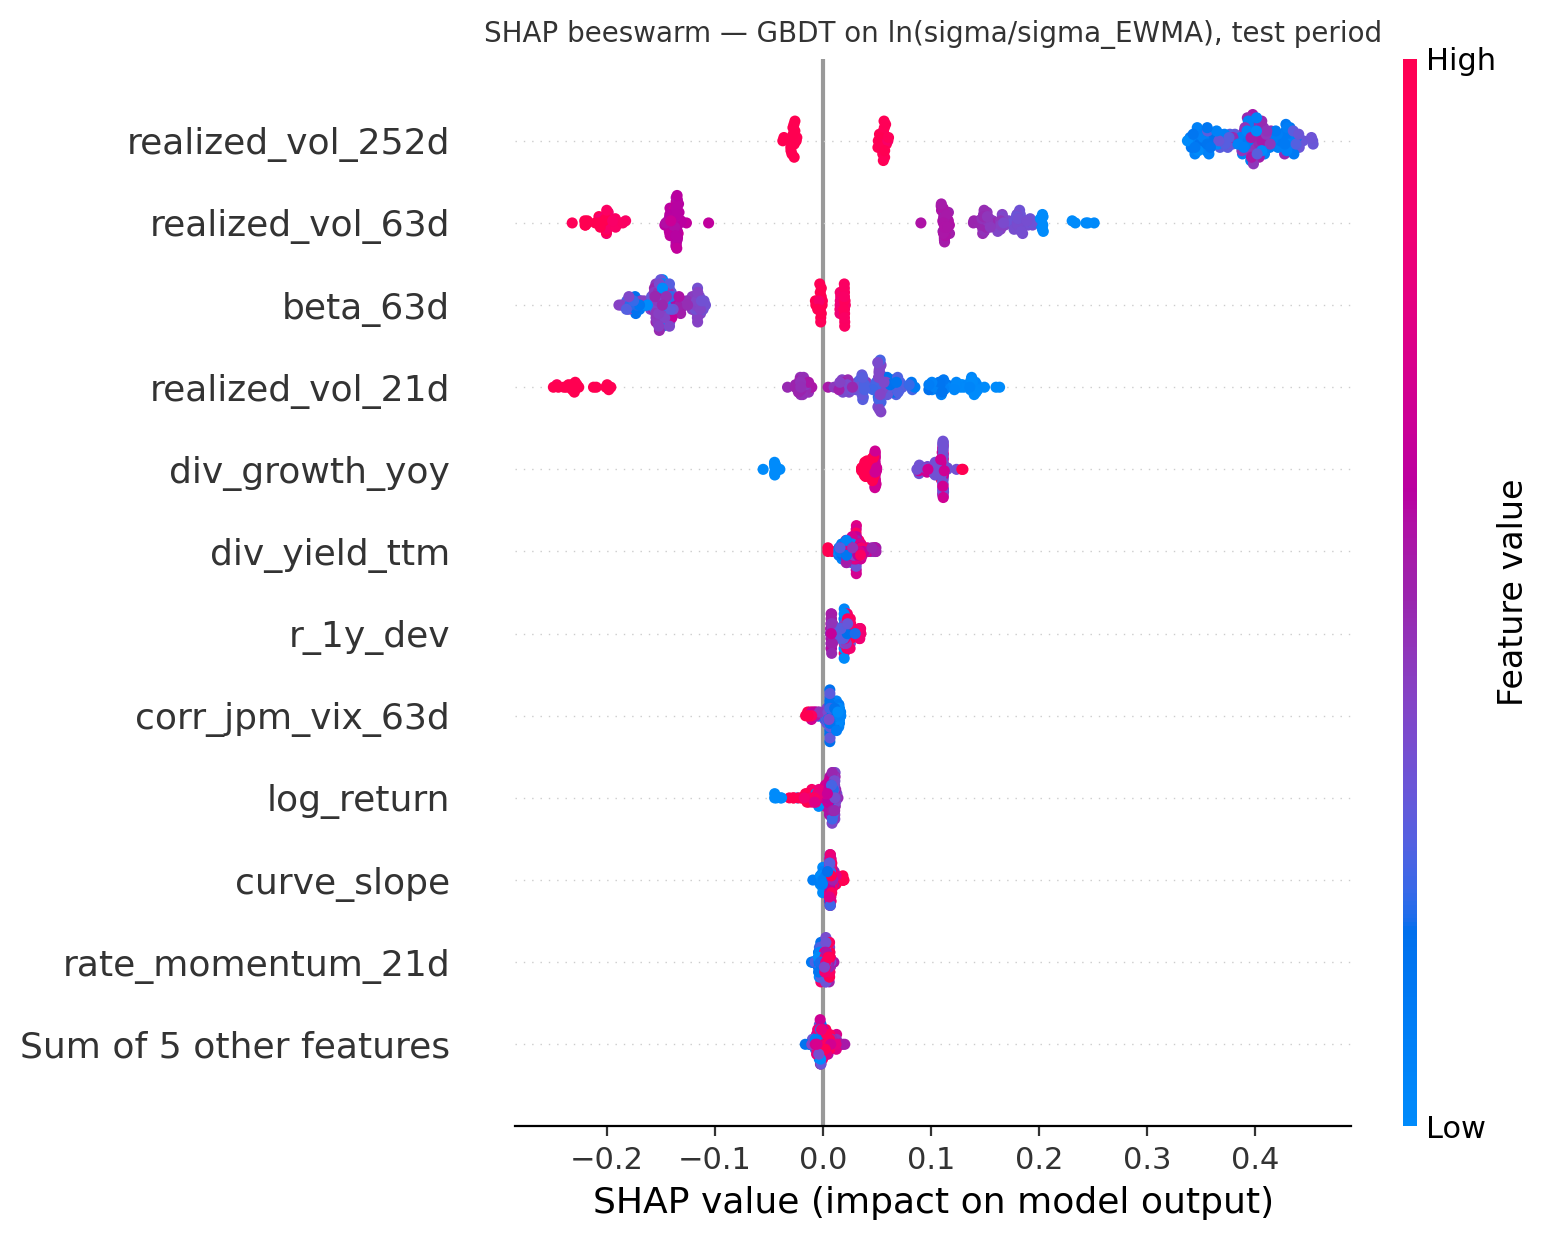
\includegraphics[width=0.66\textwidth]{../week6/figures/shap_beeswarm.png}
\caption{SHAP（部署版 GBDT，锚定目标）：长期已实现波动率主导——当前波动率低于长期水平时模型倾向正修正，干净的均值回复逻辑}
\end{figure}

\section{敏感性分析与定价工具（第 7--8 周）}
以最新市场快照（2026-08-20：$S=\$351.55$、$\sigma_{EWMA}=19.1\%$、$r=3.99\%$）做极端情景：波动率 $+50\%$ $\to$ 价格 $+48.9\%$，而加息 200bp 仅 $+1.5\%$（双腿 vega 叠加、rho 对消——波动率是 chooser 的绝对主导风险因子）；股价 $\pm15\%$ 均抬价（双向凸性）；SHAP 影响经定价函数美元化后，锚定口径下长记忆波动率主导（\texttt{realized\_vol\_252d} 一次典型贡献 $\approx+\$16.9$）。

\textbf{Streamlit 工具}（\texttt{streamlit run app/streamlit\_app.py}）：双定价（主定价 = EWMA 锚定 BSM；ML 参考价附“样本外未证优”警示）、分状态误差区间（第 4 周基准 MAE）、价格趋势、情景与压力面、历史性能指标存档、一键实时数据更新（GitHub Actions 周更为底）。全部定价逻辑位于独立服务层，六项审计通过（与闭式解逐位一致、无套利排序、情景重算、压力面单调、确定性、UI 零公式）。

\begin{figure}[H]
\centering
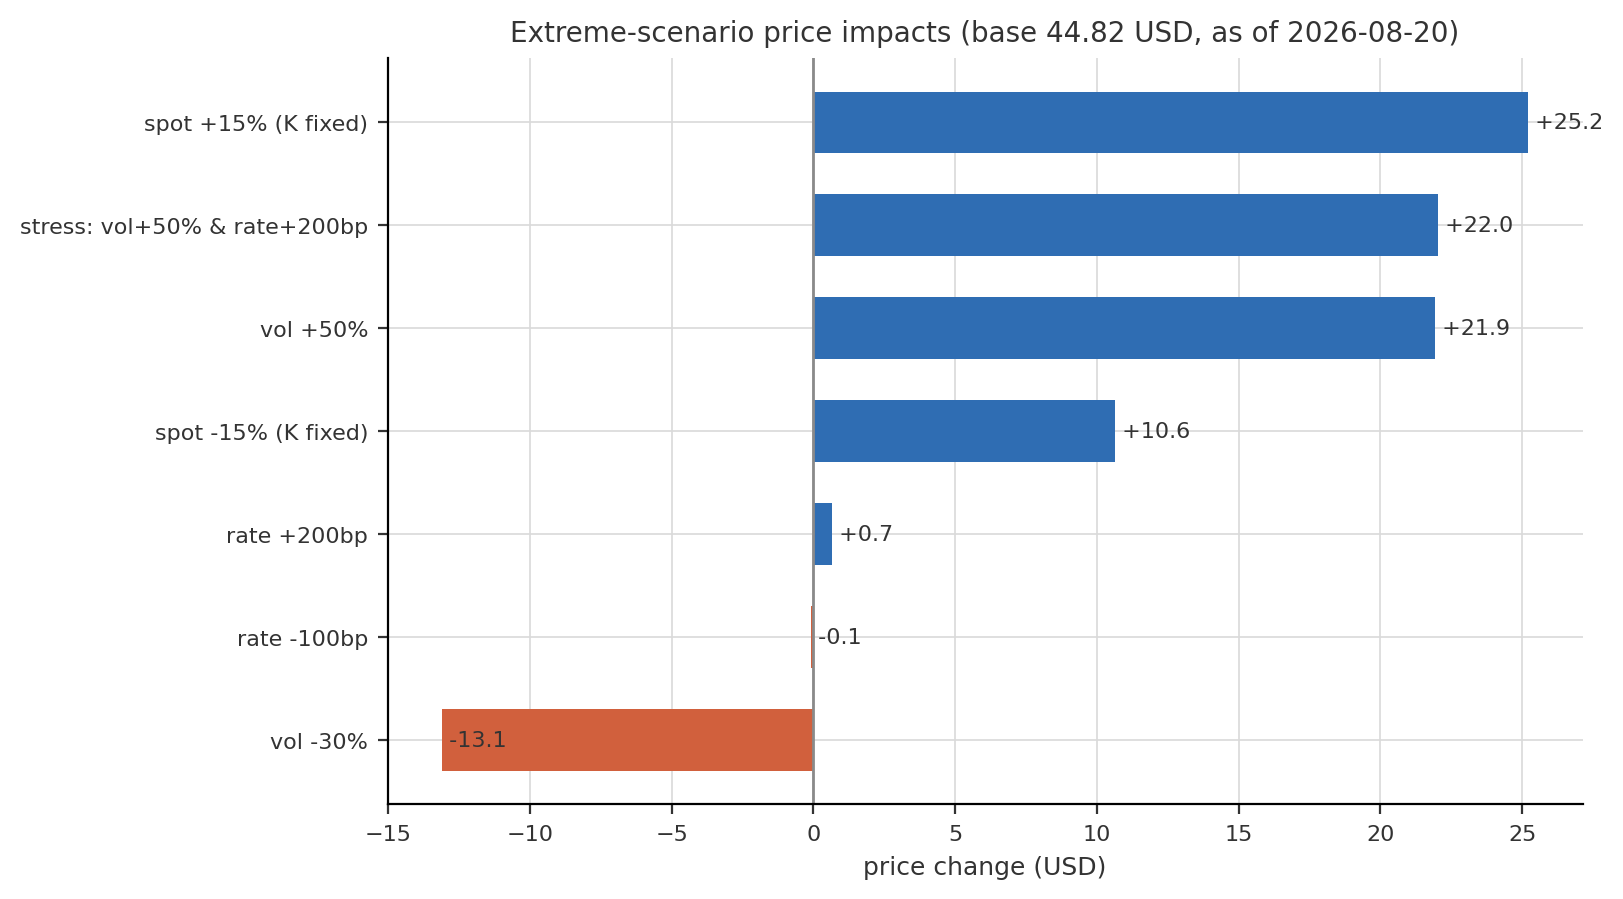
\includegraphics[width=0.74\textwidth]{../week7/figures/scenario_tornado.png}
\caption{极端情景价格冲击（2026-08-20 市场快照，基准 \$44.82）}
\end{figure}

\begin{figure}[H]
\centering
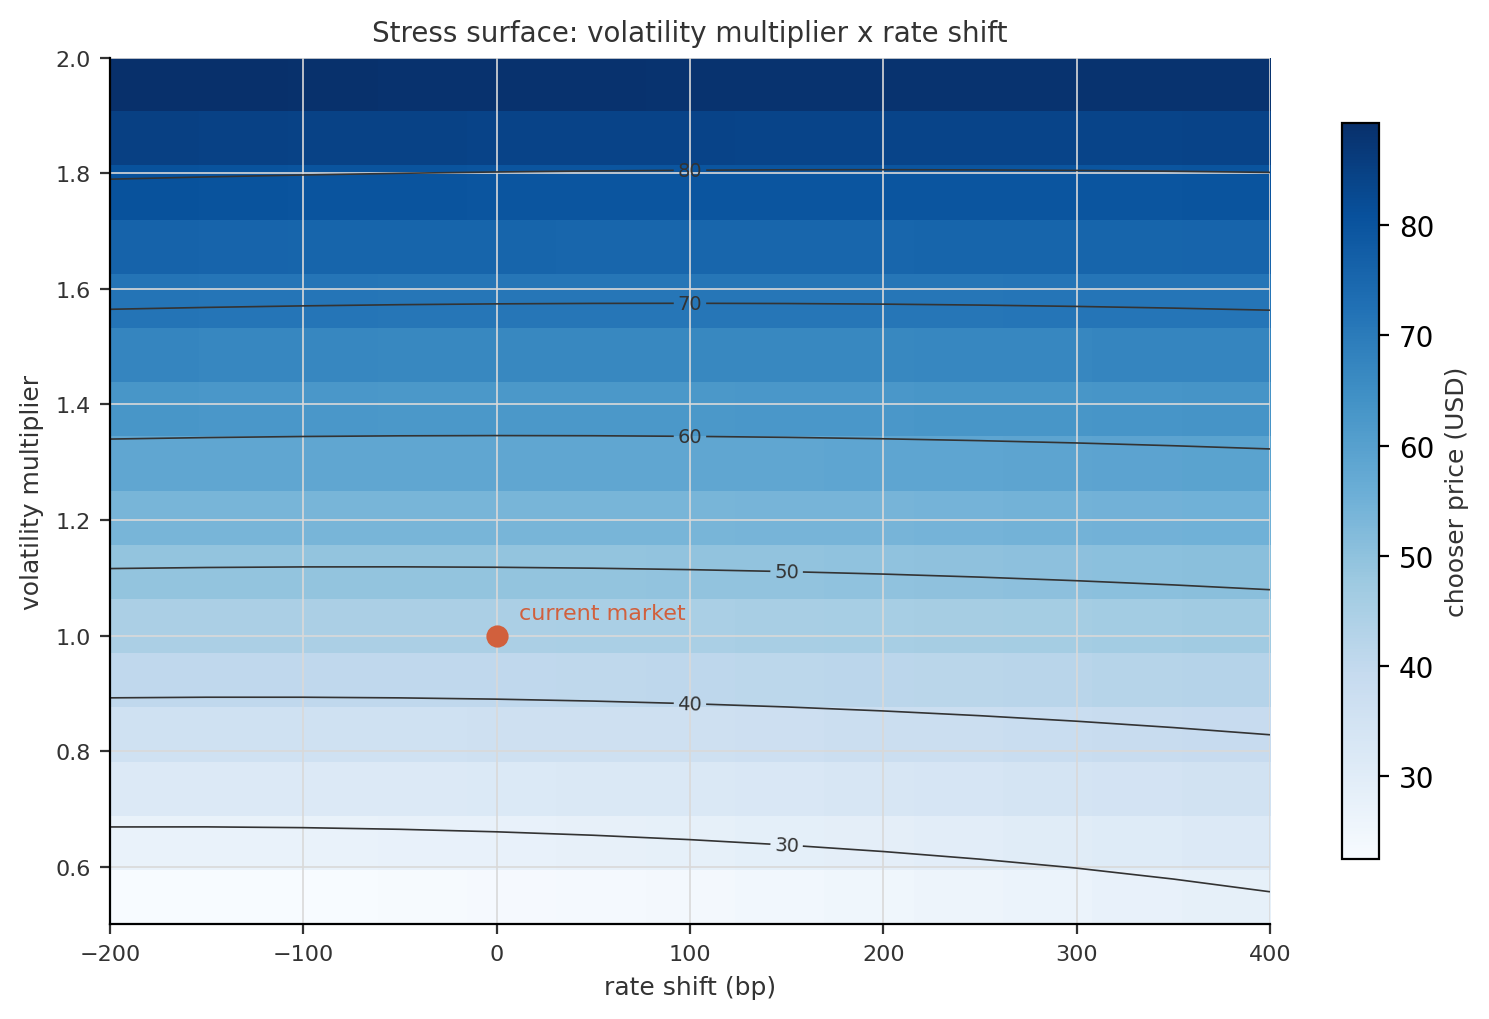
\includegraphics[width=0.68\textwidth]{../week7/figures/stress_heatmap.png}
\caption{压力曲面：波动率乘数 $\times$ 利率平移（等高线为价格）}
\end{figure}

\section{结论与展望：机器学习 $\times$ 随机过程的 1+1 融合}
本项目的全部证据指向同一个结构性结论：\textbf{随机过程与机器学习不是竞争关系，而是分工关系}——前者负责无套利框架、可对冲体系与可归因的误差结构，后者负责框架内解析方法覆盖不到的残差。据此提出五条融合路线（按可行性排序）：
\begin{enumerate}
  \item \textbf{锚定残差学习（本项目已实践）}：ML 预测 $\ln(\sigma/\sigma_{anchor})$ 而非水平，输出经 BSM 映射自动满足无套利；表现有基线下界。当前数据规模下修正幅度不可稳健标定，但框架正确——数据条件（多周期历史或个股隐含波动率）满足时即可释放；
  \item \textbf{收缩融合}：$\sigma = \sigma_{anchor}\cdot e^{\lambda \hat y}$，收缩系数 $\lambda\in[0,1]$ 由滚动验证标定——在“完全信任锚”与“完全信任 ML”之间连续插值，最坏情形受控；
  \item \textbf{状态门控校准}：ML 不直接定价，而判别当前波动率状态（平静/恐慌/转换），据此切换随机过程侧的校准窗口——直接针对第 4 周“无单一窗口全状态占优”的发现，ML 只做它擅长的分类；
  \item \textbf{隐含波动率曲面残差}：以随机过程模型（SVI/局部波动率）拟合个股期权隐含波动率曲面，ML 学习曲面残差的动态——信息含量与样本量均优于时序外推，是解除本项目数据约束的首选（需个股期权数据）；
  \item \textbf{ML 作定价加速器（surrogate）}：训练数据由随机过程模型自身生成（要多少有多少，无信噪比问题），ML 学习“参数 $\to$ 价格”映射以加速复杂模型（随机波动率、美式 chooser）的实时定价与校准——与市场有效性无冲突，工程价值确定。
\end{enumerate}
其中 4、5 与美式 chooser（Longstaff--Schwartz）共同构成 enhancement 阶段的候选方向。

\section*{附录：可复现性}
全流程固定种子、重跑逐位一致；每周交付经固定自检套餐（确定性重跑、审计断言、依赖扫描、打包泄露检查、报告数字回查）；逐周审计脚本位于 \texttt{analysis/weekN/}；一键复现入口 \texttt{python -m src.analysis\_w3} 至 \texttt{w7}；数据管道 \texttt{python -m src.collect\_all} + \texttt{src.preprocess}；部署模型 \texttt{models/final\_*.joblib}。代码仓库结构与运行说明见 README。

\section*{附录：GenAI 使用情况说明}
\textbf{使用的工具}：本项目使用 Anthropic Claude Code 作为编程与写作助手在本地终端中运行，无其他生成式 AI 工具。

\textbf{使用范围}：AI 参与了以下工作的初稿或实现：
\begin{enumerate}
  \item 代码实现：数据采集与清洗脚本、BSM 与 chooser 定价模块、蒙特卡洛验证、评估指标模块、机器学习训练与 walk-forward 协议、情景引擎、Streamlit 工具及各周审计脚本；
  \item 文档排版与初稿：周报、学习报告、各周技术文档、最终报告、演示幻灯的 LaTeX 与 pptx 生成，以及图表绘制脚本；
  \item 工程辅助：调试、依赖检查、交付物打包、格式修正（如中文标点统一、拼写标记清理）、录屏拼接。
\end{enumerate}

\textbf{由本人完成的部分}：
\begin{enumerate}
  \item 参考资料的选择：除了导师推荐的书目外，还新添了自己学过看过的一些随机过程、时间序列、数值方法等的书籍作为参考；
  \item 问题定义与阶段规划：在给定的框架下确定每周的具体范围与推进节奏；
  \item 关键方法的提出或决策：验证方式改为蒙特卡洛和情绪数据改用 VIX（这两者由本人提出并交给导师拍板）、锚定目标的采纳、测试集只开封一次的协议、第六周负结果的如实报告（而非继续调参）等；
  \item 与导师的全部沟通，以及根据导师反馈对方向和材料形态的调整；
  \item 结果审查：对 AI 产出的代码逻辑、报告数字与图表口径逐项核对，发现并要求修正过多处不一致（如第八周幻灯中的图表与讲述口径的不一致、报告图表数量不足等）；
  \item 演示视频的讲解与录制，以及学习报告初版（项目启动前撰写的那部分）中的问题设定。
\end{enumerate}

\textbf{质量控制方式}：为了防止 AI 生成内容引入错误，本项目建立了固定的自检流程：
\begin{itemize}
  \item 每周所有分析脚本都使用固定的随机种子重跑并逐位比对；
  \item 每周编写独立的审计脚本、检查重要的性质（如闭式解与蒙特卡洛一致、锚定模型输出零时恒等于基线、工具与研究代码统一口径）；
  \item 用静态扫描核对依赖列表；
  \item 将报告中的每个数字都回查到生成它的脚本输出（两套独立实现的闭式解在 $7\times10^{-15}$ 精度上一致就是这一流程的一个例子）。
\end{itemize}

\section*{参考文献}
\begin{enumerate}
  \item Huang, Z., Wang, X., Wan, W. (2021). \textit{Exploration of JPMorgan Chooser Option Pricing}. BCP Business \& Management, Vol.~15, 93--102.（复现对象）
  \item Rubinstein, M. (1991). \textit{Options for the Undecided / Exotic Options}.（simple chooser 闭式解）
  \item Hull, J., White, A. (1987). \textit{The Pricing of Options on Assets with Stochastic Volatilities}. Journal of Finance.（常数波动率局限）
  \item Gu, S., Kelly, B., Xiu, D. (2020). \textit{Empirical Asset Pricing via Machine Learning}. RFS.（金融 ML 方法论）
  \item Bakshi, G., Cao, C., Chen, Z. (1997). \textit{Empirical Performance of Alternative Option Pricing Models}. Journal of Finance.（替代模型基准）
  \item Hull, J. \textit{Options, Futures, and Other Derivatives}，11th ed.（理论底本）
\end{enumerate}
\end{document}
